\documentclass[tikz,border=4pt]{standalone}
\usepackage{amsmath}
\begin{document}
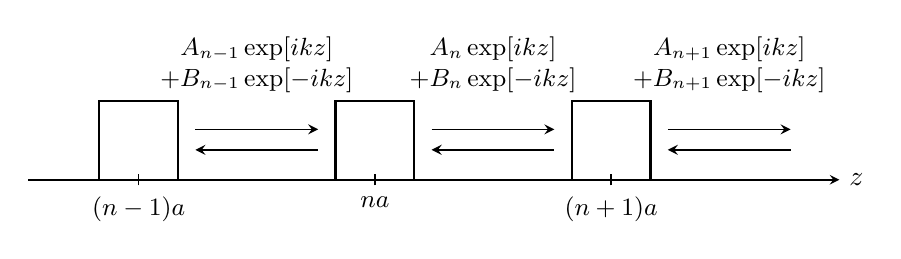
\begin{tikzpicture}[>=stealth, thick, scale=1.0]
  % z-axis
  \draw[->, line width=0.55pt] (-4.4, 0) -- (5.9, 0) node[right] {$z$};

  % Three periodic barriers centered at x = -3.0, 0.0, 3.0 (period a = 3.0, width b = 1.0)
  \foreach \xc/\lbl in {-3.0/$(n-1)a$, 0.0/$na$, 3.0/$(n+1)a$} {
    \draw[line width=0.85pt] (\xc - 0.5, 0) rectangle (\xc + 0.5, 1.0);
    \draw[line width=0.5pt] (\xc, -0.07) -- (\xc, 0.07);
    \node[below, font=\small] at (\xc, -0.08) {\lbl};
  }

  % Arrows in free regions
  \foreach \xm in {-1.5, 1.5, 4.5} {
    \draw[->, line width=0.6pt] (\xm - 0.78, 0.64) -- (\xm + 0.78, 0.64);
    \draw[<-, line width=0.6pt] (\xm - 0.78, 0.38) -- (\xm + 0.78, 0.38);
  }

  % Labels above free regions
  \node[above, align=center, font=\small] at (-1.5, 0.98) {$A_{n-1}\exp[ikz]$ \\ $+ B_{n-1}\exp[-ikz]$};
  \node[above, align=center, font=\small] at (1.5, 0.98) {$A_n\exp[ikz]$ \\ $+ B_n\exp[-ikz]$};
  \node[above, align=center, font=\small] at (4.5, 0.98) {$A_{n+1}\exp[ikz]$ \\ $+ B_{n+1}\exp[-ikz]$};
\end{tikzpicture}
\end{document}
